\chapter{Detecção facial}\label{cap:detecao_facial}

%\chapterprecis{Definição, utilidade, requisitos, dificuldades e métodos.}

O papel de um detector de faces é, dada uma imagem arbitrária, determinar se ela contém faces humanas ou não e, caso positivo, retornar a localização e dimensões de cada face \cite{censtudy}.

A detecção de faces é utilizada em câmeras fotográficas para ajuste automático de foco, em softwares de imagens e redes sociais para marcação de pessoas e é uma etapa importante para o processo de reconhecimento facial. Antes de executar um algoritmo de reconhecimento facial, é de praxe realizar uma detecção facial a fim de concentrar os esforços do reconhecedor facial apenas nas áreas relevantes.

É preciso minimizar tanto a quantidade de faces não identificadas (falso-negativos) quanto objetos reconhecidos erroneamente como faces (falso-positivos) para obter uma performance aceitável. Para tanto, algoritmos de aprendizado de máquina podem ser muito úteis.

Diversas dificuldades influenciam na eficiência dos algoritmos, como ruídos, variação de iluminação, expressões faciais, imagem de fundo, orientação da cabeça, obstrução da face ou sobreposição de faces \cite{de2015processo} e, nota-se que, para análise de streamings de vídeo, é fundamental que a detecção facial seja realizada em tempo real.

\section{Métodos}

Segundo \citeonline{de2015processo}:

\begin{citacao}
As técnicas mais citadas para realizar a detecção de faces são: casamento de padrões que consiste na detecção por meio de comparações com formas geométricas, modelos estatísticos, modelos baseado em redes neurais, modelos baseados em tons de pele e o Viola-Jones.
\end{citacao}

\citeonline{yang2002detecting} classificou os algoritmos de detecção e reconhecimento facial em quatro categorias:


\begin{enumerate}
\item \textbf{Métodos baseados em conhecimento (\textit{knowledge-based})} -- Utilizam regras baseadas no conhecimento sobre características das faces humanas, como posição dos olhos e simetria. Este método possui a desvantagem de ser difícil derivar regras precisas que cubram todos os cenários.

\item \textbf{Métodos baseados em características (\textit{feature based})} -- Procuram características invariantes que definam uma face, como regiões com cor de pele, formato dos lábios e bochechas. São bastante impactados por sombras e ruídos.

\item \textbf{Métodos de casamento de padrões (\textit{template matching})} -- Utilizam templates predefinidos de faces, como uma silhueta ou um mapa de bordas. Este método não lida bem com variações de escala, poses, orientação e formatos de rosto.

\item \textbf{Métodos baseados na aparência (\textit{appearance-based})} -- Utilizam algoritmos de aprendizado de máquina e bancos de imagens para treinar classificadores. Este é o método mais bem sucedido.

\end{enumerate}


\begin{table}[htbp]
\centering
\caption{Categorias de métodos para detecção facial segundo \citeonline{yang2002detecting}}
\label{tab:categoria_trabalhos}
\begin{tabular}{@{}ll@{}}
\toprule
\multicolumn{1}{c}{\textbf{Abordagem}}                  & \multicolumn{1}{c}{\textbf{Trabalhos representativos}}\\\midrule
\multicolumn{2}{l}{\textbf{Baseados em conhecimento}}                                                           \\\midrule
                                                        & \citeonline{yang1994human}                            \\\midrule
\multicolumn{2}{l}{\textbf{Características invariantes}}                                                        \\\midrule
\multirow{2}{*}{\hspace{3mm}-- Características faciais} & \citeonline{leung1995finding}                         \\\cmidrule(l){2-2} 
                                                        & \citeonline{yow1997feature}                           \\\midrule
\hspace{3mm}-- Textura                                  & \citeonline{dai1996face}                              \\\midrule
\multirow{2}{*}{\hspace{3mm}-- Cor da pele}             & \citeonline{yang1996real}                             \\\cmidrule(l){2-2} 
                                                        & \citeonline{mckenna1998modelling}                     \\\midrule
\hspace{3mm}-- Múltiplas características                & \citeonline{kjeldsen1996finding}                      \\\midrule
\multicolumn{2}{l}{\textbf{Casamento de padrões}}                                                               \\\midrule
\hspace{3mm}-- Templates predefinidos                   & \citeonline{craw1992finding}                          \\\midrule
\hspace{3mm}-- Templates deformáveis                    & \citeonline{lanitis1995automatic}                     \\\midrule
\multicolumn{2}{l}{\textbf{Baseados na aparência}}                                                              \\\midrule
\hspace{3mm}-- Eigenface                                & \citeonline{turk1991eigenfaces}                       \\\midrule
\hspace{3mm}-- Baseado em distribuição                  & \citeonline{sung1998example}                          \\\midrule
\hspace{3mm}-- Redes neurais                            & \citeonline{rowley1998neural}                         \\\midrule
\hspace{3mm}-- Máquina de vetores de suporte  (SVM)     & \citeonline{osuna1997training}                        \\\midrule
\hspace{3mm}-- Classificador Naive Bayes                & \citeonline{schneiderman1998probabilistic}            \\\midrule
\hspace{3mm}-- Modelo oculto de Markov (HMM)            & \citeonline{rajagopalan1998finding}                   \\\midrule
\multirow{2}{*}{\hspace{3mm}-- Teoria da informação}    & \citeonline{lew1996information}                       \\\cmidrule(l){2-2} 
                                                        & \citeonline{collobert1996listen}                      \\\bottomrule
\end{tabular}
\end{table}

\begin{figure}[htbp]
    \caption{Exemplos de métodos de detecção facial}
    \label{fig:metodos_deteccao}
    \begin{subfigure}[t]{0.45\textwidth}
    \centering
    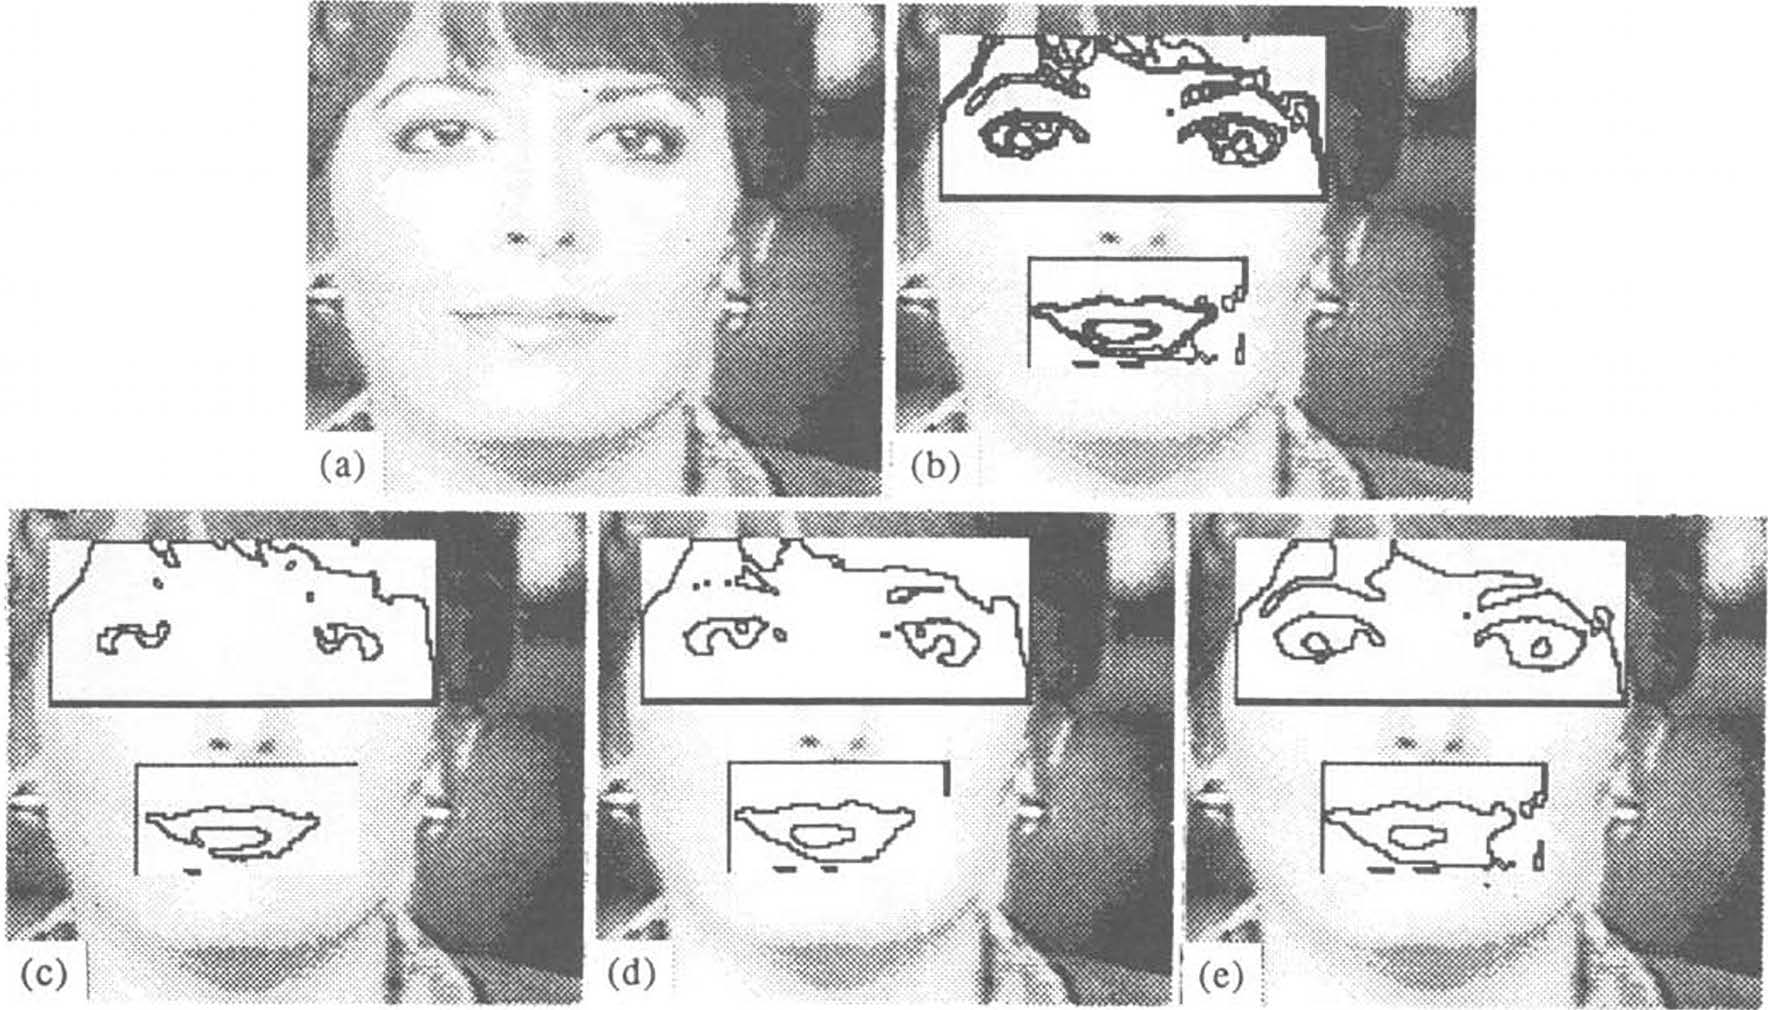
\includegraphics[width=\textwidth]{imagens/yang_edge_detection.png}
    \caption{Baseado em conhecimento. Fonte: \citeonline{yang1994human}}
    \end{subfigure}
    \hfill
    \begin{subfigure}[t]{0.45\textwidth}
    \centering
    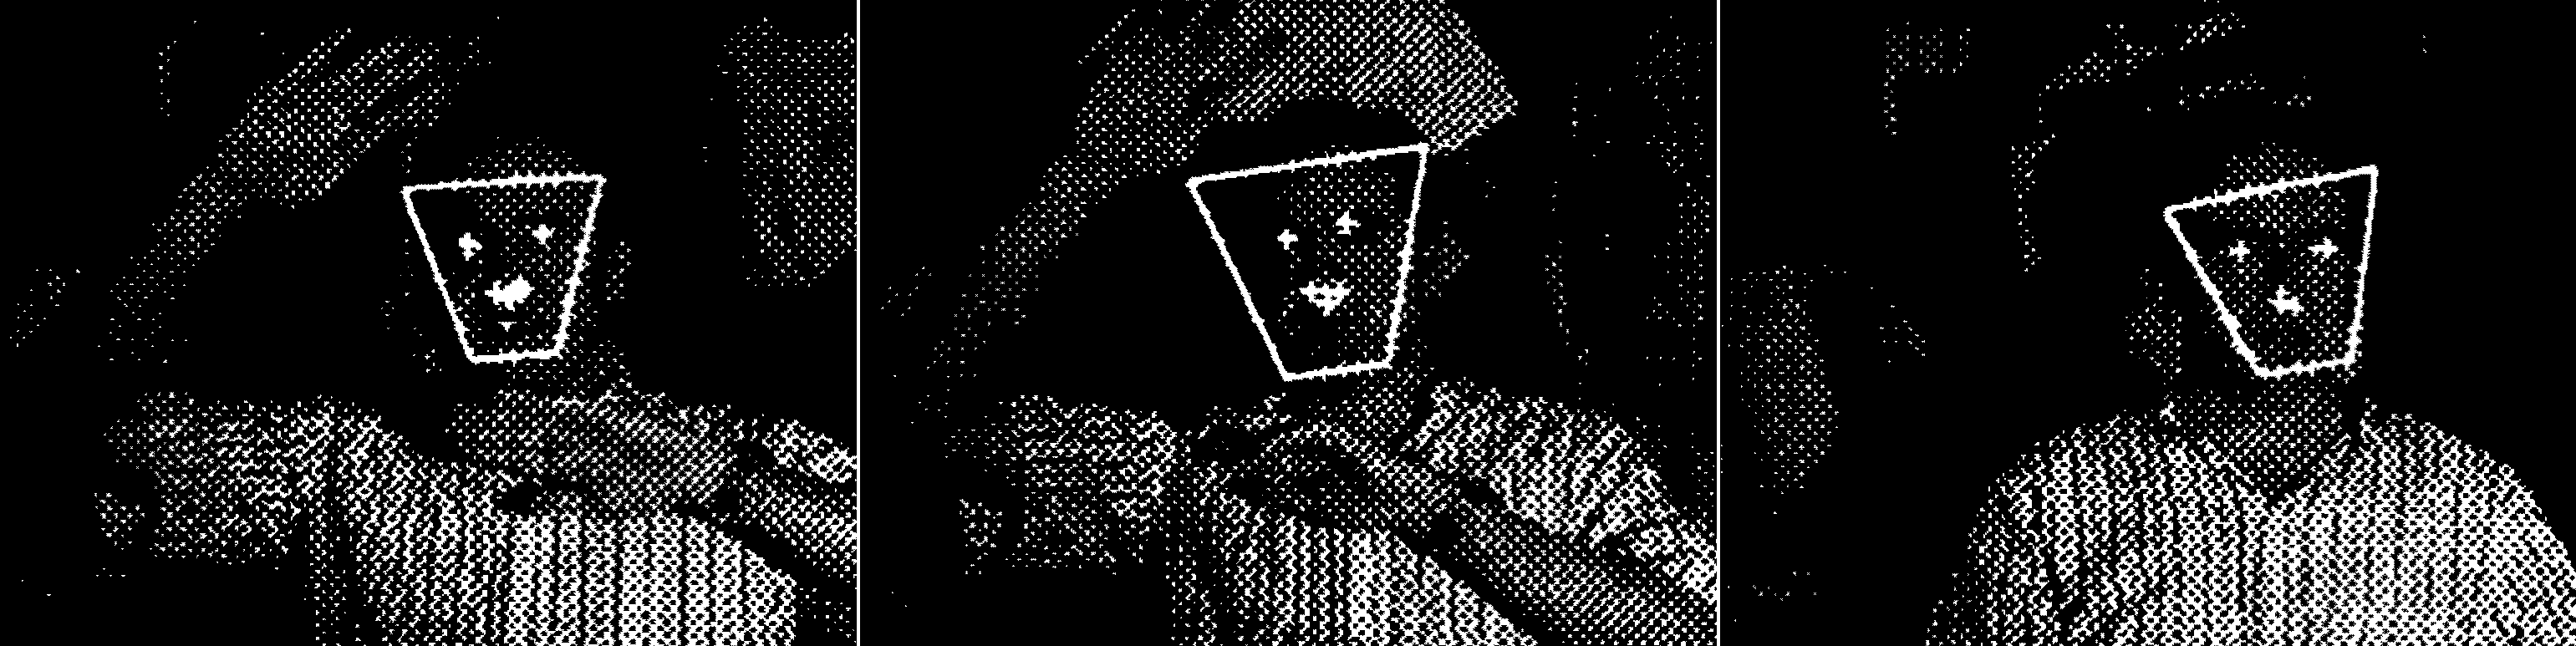
\includegraphics[width=\textwidth]{imagens/leung.png}
    \caption{Baseado em características invariantes.  Fonte: \citeonline{leung1995finding}}
    \end{subfigure}
    
    \begin{subfigure}[t]{0.45\textwidth}
    \centering
    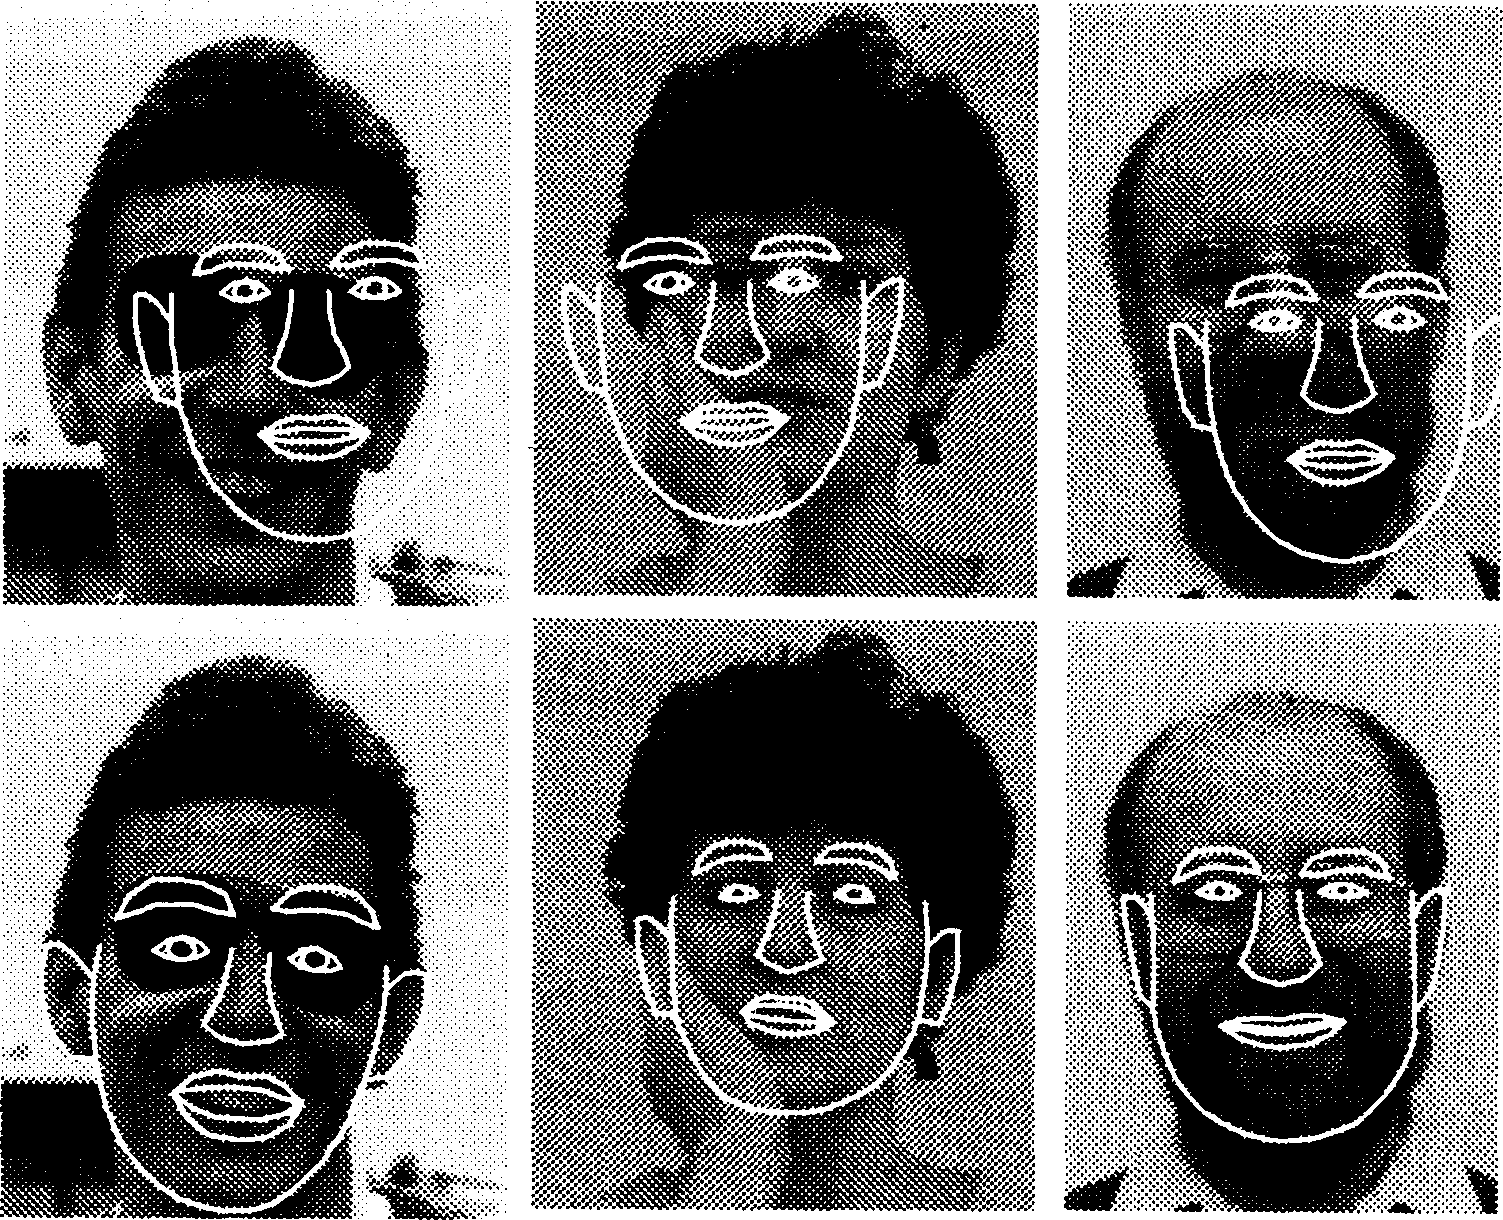
\includegraphics[width=\textwidth]{imagens/lanitis_template.png}
    \caption{Casamento de padrões. Fonte: \citeonline{lanitis1995automatic}}
    \end{subfigure}
    \hfill
    \begin{subfigure}[t]{0.45\textwidth}
    \centering
    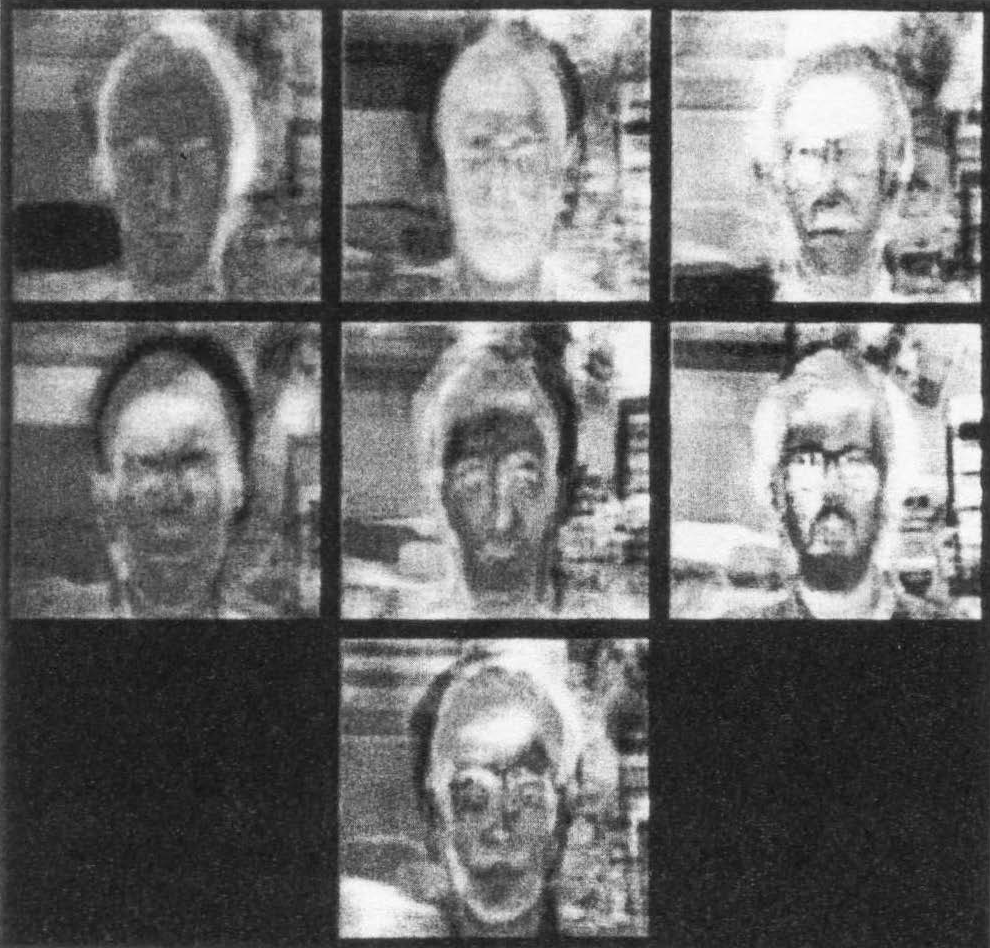
\includegraphics[width=\textwidth]{imagens/turk_eigenfaces.png}
    \caption{Baseado na aparência. Fonte: \citeonline{turk1991eigenfaces}}
    \end{subfigure}
\end{figure}